\chapter{Z Tanım Bölgesinde Kök Eğrisi}
Z tanım bölgesinde bir transfer fonksiyonu $T=0.2$ olmak üzere
\begin{equation}
    G(z)=\frac{1}{z^3 + 0.4 z^2 - 0.37 z - 0.04}
\end{equation}
olarak verilmiştir. P kontrolör ile kapalı çevrim transfer fonksiyonu
\begin{equation}
\begin{split}
    T(z)&=\frac{kG(z)}{1+kG(z)}\\
    T(z)&=\frac{\frac{k}{z^3 + 0.4 z^2 - 0.37 z - 0.04}}{1+\frac{k}{z^3 + 0.4 z^2 - 0.37 z - 0.04}}\\
    T(z)&=\frac{k}{z^3 + 0.4 z^2 - 0.37 z - 0.04+k}
\end{split}
\end{equation}
olarak hesaplanır. Karakteristik polinomunda $k$ değiştikçe köklerin aldığı değer Çizelge~\ref{tbl:lec5_rlocus1} ile verilmiştir. Her kutbun kendi hareketinin görselleştirildiği çizime \textbf{Kök Eğrisi} denir. Sisteme ait kök eğrisi Şekil~\ref{fig:lec5_rlocus1} ile verilmiştir.

\setlength{\tabcolsep}{30pt}
\renewcommand{\arraystretch}{1}
\begin{table}[!htb]
    \caption{$k$'nın değişimine göre polinomun köklerinin yada sistem kutuplarının değişimi}\label{tbl:lec5_rlocus1}
    \begin{tabularx}{\textwidth}{cccc}\hline
    $\mathbf{k}$& $\mathbf{z_1}$& $\mathbf{z_2}$& $\mathbf{z_3}$\\\hline
    0.1& -0.8909& 0.2455 + 0.0843i&  0.2455 - 0.0843i\\
    0.2& -0.9594& 0.2797 + 0.2975i&  0.2797 - 0.2975i\\
    0.3& -1.0160& 0.3080 + 0.4013i&  0.3080 - 0.4013i\\
    0.4& -1.0649& 0.3325 + 0.4770i&  0.3325 - 0.4770i\\
    \vdots& \vdots& \vdots& \vdots\\\hline
    \end{tabularx}
\end{table}

\begin{figure}[!htb]
    \centering
    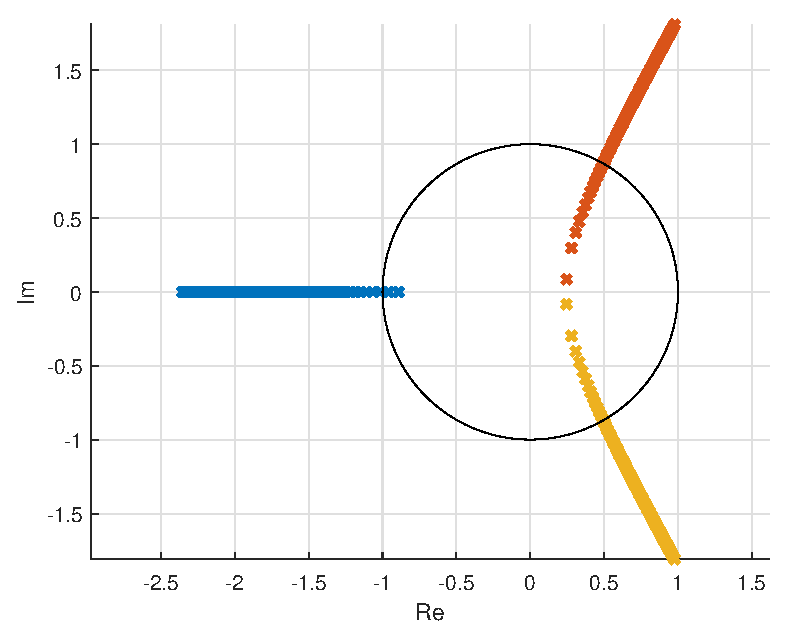
\includegraphics[width=0.75\textwidth]{img/lec5_rlocus1}
    \caption{Sisteme ait kök eğrisi}
    \label{fig:lec5_rlocus1}
\end{figure}

Şekil~\ref{fig:lec5_rlocus1} ile verilen ayrık noktalar birleştirildiğinde Şekil~\ref{fig:lec5_rlocus2} oluşmaktadır.
\begin{figure}[!htb]
    \centering
    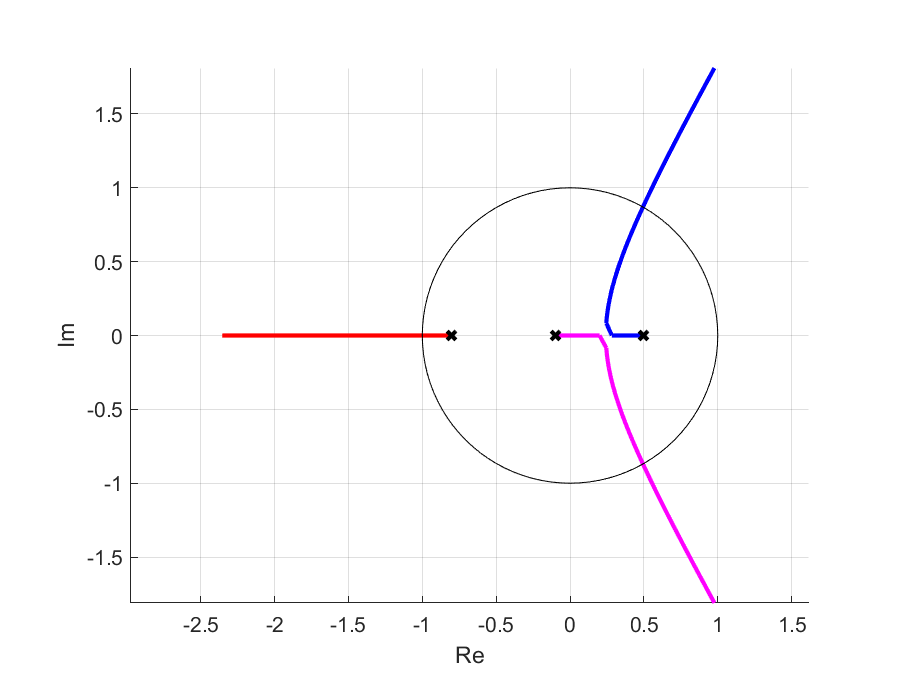
\includegraphics[width=0.75\textwidth]{img/lec5_rlocus2}
    \caption{Sisteme ait kök eğrisi}
    \label{fig:lec5_rlocus2}
\end{figure}

S tanım bölgesinde kararlılık sınırı $s=jw$ ile elde edilmektedir ve bu durumda $\zeta=0$'dır. Dolayısıyla,
\begin{equation}
\begin{split}
    y(t)&=1-e^{-\zeta w_nt}\left[\cos(\sqrt{1-\zeta^2}w_nt)+\frac{\zeta}{\sqrt{1-\zeta^2}}\sin(\sqrt{1-\zeta^2}w_nt)\right]\\
    &=1-\cos(w_nt)
\end{split}
\end{equation}
elde edilmektedir. Görüldüğü üzere sistem yanıtı salınımlıdır. Girişe uygulanan birim basamak sinyaline karşın sistem salınım yapmakta ve giriş sinyali değerine yakınsamamaktadır. Z tanım bölgesine $z=e^{sT}$ ile geçiş yapılırsa
\begin{equation}
    \begin{split}
        z&=e^{iwT}\\
        z&=e^{i\theta}\\
        z&=1\phase{ \theta}
    \end{split}
\end{equation}
elde edilir. Dikkat edilirse açı değişmekte fakat genlik sabittir ve bu ifade birim çemberi tanımlamaktadır. 
